% Main manuscript for Nondestructive Testing and Evaluation.
% Taylor & Francis Interact layout with NLM numbered references.
\documentclass[]{interact}

\usepackage{epstopdf}
\usepackage[caption=false]{subfig}
\usepackage[numbers,sort&compress]{natbib}
\bibpunct[, ]{[}{]}{,}{n}{,}{,}
\renewcommand\bibfont{\fontsize{10}{12}\selectfont}
\usepackage{url}
\usepackage{float}
\usepackage{array}

\newcolumntype{L}[1]{>{\raggedright\arraybackslash}p{#1}}

\graphicspath{{figures/}}

\begin{document}

\articletype{RESEARCH ARTICLE}

\title{Provenance-aware evaluation of ground-penetrating-radar recognition reveals fragile cross-environment generalization}

\author{
\name{Zixuan Liu\textsuperscript{a} and Wei Xiong\textsuperscript{b,c}\thanks{CONTACT Wei Xiong. Email: xw@mail.hbut.edu.cn}}
\affil{\textsuperscript{a}Detroit Green Technology Institute, Hubei University of Technology, Wuhan 430068, China; \textsuperscript{b}School of Electrical and Electronic Engineering, Hubei University of Technology, Wuhan 430068, China; \textsuperscript{c}Department of Computer Science and Engineering, University of South Carolina, Columbia, SC 29201, USA}
}

\maketitle

\begin{abstract}
Ground-penetrating radar (GPR) recognition models are often evaluated on curated splits that can blur class recognition with acquisition setting, provenance and environment structure. We assembled GPR-ProvenanceBench to separate executable assets, grouped-split logic and model comparisons before interpretation. The clearest and most reproducible result came from Res-SAM environment transfer: balanced accuracy fell from 0.8483 \(\pm\) 0.0308 within real-world data to 0.4367 under synthetic-to-real transfer, and from 0.9067 \(\pm\) 0.0279 within synthetic data to 0.3511 under real-to-synthetic transfer. The same direction appeared across a five-family synthesis built from HOG+RBF-SVM, a lightweight CNN, ResNet18, EfficientNetB0 and DeiT-Tiny. Mojahid showed smaller but statistically stable split sensitivity, while 4TU served as a stress test and feasibility boundary rather than a main confirmation result. Simple calibration and train-only repair mostly changed confidence or only partly reduced the gap, but did not remove the transfer effect. By combining file manifests, source-group partitions, duplicate checks and transfer tests, GPR-ProvenanceBench provides a practical route for reporting what kind of generalization a public GPR benchmark actually measures.
\end{abstract}

\begin{keywords}
ground-penetrating radar; nondestructive evaluation; data provenance;
domain shift; cross-environment transfer; generalization; benchmark
\end{keywords}

\section{Introduction}

Reliable ground-penetrating radar (GPR) recognition matters in nondestructive evaluation because its outputs are often used as evidence about buried structure, not just as classification scores. In road assessment, bridge inspection, pavement characterization and moisture-related diagnosis, the practical question is not only whether a model can separate classes, but whether the output stays trustworthy when the acquisition setting, preprocessing route or measurement geometry changes. That concern is visible across recent journal examples in Nondestructive Testing and Evaluation, where GPR is used for runway compaction, pavement thickness, bridge inspection, structural-needs assessment and moisture detection, and where other NDE modalities are increasingly coupled with deep learning, vision, thermography and ultrasonic analysis \cite{cheng2023runway,hu2016pavement,benedetto2012bridges,plati2012structural,kilic2014moisture,rathod2024uav,ibrahim2024thermography,qu2024impactecho}. The literature here is mostly about applied validation, so the real question is whether a given workflow remains reliable when it is tested outside the exact data organization on which it looked good.

At the same time, the literature tends to be task-specific. Many studies evaluate a single defect class, a single infrastructure type or a single local validation setting, which is appropriate for application demonstration but does not by itself establish deployment reliability. Some papers emphasize signal-processing refinements or physical interpretation \cite{economou2012deconvolution,lualdi2014polarisation,artagan2022thermal,wang2024tracer,dong2024vibrometry}, while others compare detectors, neural networks or post-processing pipelines within one dataset \cite{cheng2023runway,wang2024crack,kilic2014moisture,rathod2024uav,nategh2024kmeans,li2024pinn}. These studies are useful, but they usually answer a narrower question than the one needed for reliable use: what happens when the apparent signal is re-evaluated under a different provenance structure or acquisition environment? Put differently, most prior work asks whether GPR can solve a local task, whereas the present question is whether a reported score still means the same thing once the sample organization changes. That is why a split that ignores provenance can look convincing on paper and still be a poor proxy for deployment.

That distinction matters because GPR sample structure can be entangled with provenance. Site identity, project identity, acquisition route, rendering choices and preprocessing steps may all carry information that is helpful for in-split prediction but misleading for deployment. If the split protocol does not respect those structures, then high internal performance can reflect a mixture of target signal and acquisition-specific regularities. In that case, a random split is not just convenient; it can be a weak test of generalization. The unresolved challenge is therefore not whether GPR can work on curated data, but how to tell whether a reported score still holds when the data are reorganized in a way that matches actual use. This is the point at which a performance paper has to become a reliability paper.

This problem is especially visible for public GPR assets. Public files are often released after several processing steps, such as cropping, B-scan rendering, class sorting, augmentation, re-exporting or conversion from raw traces to image matrices. Those steps are useful because they make data sharable and make model training possible, but they can also create related samples that are easy to split incorrectly. An augmented image can sit in the test set while its parent image sits in the training set. Two byte-identical or visually identical files can be treated as independent examples. Samples collected from the same project or environment can be distributed across both sides of a random split. In all three cases, the classifier is tested against a partly familiar data organization. The result may still be reproducible, but it no longer answers the same question as a source-separated or environment-separated test.

To address this gap, we built GPR-ProvenanceBench as a reproducible evaluation workflow rather than a single benchmark table. Each asset is first assigned an executable status, then compared under split, transfer, stress-test and repair settings, and finally interpreted only within the evidence boundary that the asset can actually support. This design keeps grouped evaluation, cross-environment transfer and blind external validation separate, and makes the role of each asset explicit. Some assets support the main claim, while others are only useful as stress tests or boundary checks.

The design follows a simple principle. A benchmark should first say what the samples are, where they came from and how they are related, and only then compare model scores. This order differs from the common model-first workflow, in which a dataset is loaded, split and scored before its source structure is inspected. In GPR, reversing that order matters because the same image label can be connected to acquisition environment, project identity, survey route, trace processing and augmentation history. GPR-ProvenanceBench therefore treats the split manifest as part of the experimental result. The manifest records which samples were allowed to share a partition, which samples were deliberately separated and which sample relationships could not be resolved from the public files.

The paper uses that framework to ask whether provenance-aware evaluation changes the reliability picture for GPR recognition. Res-SAM provides the strongest transfer-fragility signal, Mojahid offers secondary split-sensitivity evidence, and 4TU defines the stress-test boundary. The aim is not to claim universal failure, but to show where the evidence supports deployment caution and where further validation remains necessary. The practical contribution is a way to separate apparent recognition performance from the provenance structure that can drive it, so that a paper can say not only how well a GPR model performs, but what kind of evaluation is needed before that performance can be trusted.

\section{Related work}
GPR-based nondestructive evaluation has developed mainly through application-specific measurement and interpretation workflows. Field studies have used GPR to assess runway compaction, pavement thickness and structural needs, bridge condition, and asphalt quality, with validation organized around the engineering quantity or defect of interest \cite{cheng2023runway,hu2016pavement,plati2012structural,benedetto2012bridges,poikajarvi2012road}. The same application-driven style is visible in recent NTE studies of concrete crack depth, bridge debonding, thermography, laser vibrometry, guided sensing and impact-echo classification \cite{wang2024tracer,liu2024debonding,ibrahim2024thermography,dong2024vibrometry,cheng2024fusion,qu2024impactecho}. This body of work established NDE as a practical inspection technology and defined strong task-level evaluation patterns: measurements are collected in a specified setting, converted into physically or empirically meaningful features, and compared with local reference observations. The resulting evidence is well suited to the target application, while the influence of site identity, acquisition route, and sample ancestry on model evaluation is usually not treated as a separate experimental variable.

A second line of research has improved the extraction and recognition of diagnostic information from GPR signals. Representative approaches include time-varying deconvolution, polarization-based target characterization, dielectric analysis of concrete damage, and neural-network classification of moisture conditions \cite{economou2012deconvolution,lualdi2014polarisation,artagan2022thermal,kilic2014moisture}. More recent learning-based systems operate directly on B-scans and combine image features, deep networks, or foundation models with GPR-specific signal structure. Res-SAM, for example, combines segmentation with reservoir-based waveform analysis and reports clear degradation when the normal-data source and the target environment are mismatched \cite{zhou2025ressam}. Similar learning-based evaluation concerns now appear across NDE image and signal tasks, including UAV road-crack classification, thermography clustering, physics-informed wavefield analysis and impact-echo classification \cite{rathod2024uav,nategh2024kmeans,li2024pinn,qu2024impactecho}. These studies move GPR recognition toward more capable and automated models. They also make the evaluation question more consequential: performance can depend not only on target characteristics, but also on how acquisition environments and data sources are represented in training and testing.

NTE articles also tend to spend substantial space on the measurement route, the material condition and the engineering interpretation of the output. For pavement and bridge work, this often means documenting the inspection setting, the sensor configuration, the reference measurement and the way the GPR response is converted into a decision-relevant quantity \cite{hu2016pavement,plati2012structural,benedetto2012bridges,liu2024debonding,ibrahim2024thermography}. For data-driven NDE, the same expectation extends to image formation, post-processing, model input and validation design \cite{rathod2024uav,nategh2024kmeans,cheng2024fusion,qu2024impactecho}. That style is important for the present study because a benchmark paper has an analogous burden. The classifier is not the only object that needs to be described. The data release, the file lineage, the split rule and the environment separation also need enough detail for another group to reproduce the evaluation. Without that detail, a high score is hard to compare across papers, even when the model architecture and metric are reported.

In parallel, machine-learning research has established data organization as part of experimental design. Controlled leakage studies show that feature processing, repeated samples, and non-independent train--test partitions can change both predictive performance and interpretation, with effects that vary across leakage mechanisms \cite{rosenblatt2024leakage,kapoor2023leakage}. Broader validation studies have made the same point in small-sample and applied imaging settings, where leakage, underspecification and weak validation can inflate confidence in a model \cite{vabalas2019validation,roberts2021pitfalls,damour2022underspecification}. Similarity-aware splitting methods such as DataSAIL formalize the separation of related samples and combine leakage reduction with class-balanced partitioning for out-of-distribution evaluation \cite{joeres2025datasail}. This work provides a rigorous basis for split-aware model assessment. GPR, however, adds domain-specific provenance structures, including survey site, project lineage, antenna and acquisition settings, preprocessing route, synthetic--real origin, duplication, and augmentation ancestry. Evaluating these structures requires more than applying a single grouped split after model development.

The issue is related to, but not identical with, standard domain adaptation or data leakage. Domain adaptation usually starts from a known source--target pair and asks how to improve target performance. Leakage analysis often asks whether information from the test set has entered training through features, preprocessing or sample overlap. GPR provenance combines both concerns. A source group can behave like a domain, an augmentation lineage can behave like a leakage channel, and a duplicate can make a nominally independent test sample familiar to the model. The same asset may therefore need several tests before its score can be interpreted. This is why the present work evaluates environment transfer, group separation, duplicate handling, perturbation response and repair controls in one protocol family.

GPR-ProvenanceBench connects these research lines in one auditable evaluation framework. It first represents each data asset through an executable provenance record, then measures source and environment predictability, compares random and grouped splits, performs bidirectional cross-environment transfer, and introduces duplicate, augmentation, and perturbation stress tests. The same protocol family is examined across multiple model families and followed by train-only repair and calibration controls. The contribution is therefore an evaluation method rather than another recognition architecture: it produces a provenance-conditioned account of where GPR performance is stable, where model ranking changes, and where cross-environment transfer becomes the dominant reliability constraint.

This framing also defines the intended comparison with prior GPR work. The benchmark does not replace physics-based interpretation, site-specific calibration or engineering validation. It supplies the missing layer between a public dataset and a reported recognition score. In that layer, the first question is not which model is most accurate, but whether the train--test relationship matches the claim being made. A paper claiming within-asset recognition can use a different split from a paper claiming source-separated recognition or cross-environment transfer. Making those claims explicit is the main step that GPR-ProvenanceBench adds to the current literature.

\section{Materials and methods}

\subsection{Data and provenance records}

The main image analyses used the Mojahid and Res-SAM collections. Mojahid contained 2,524 B-scan images from three classes: cavity ($n=632$), intact ($n=975$) and utility ($n=917$). The manifest linked these images to 692 augmentation lineages and recorded whether each image was an original or an augmented derivative. Res-SAM contained 1,050 published image exports, including 600 real-world and 450 synthetic samples \cite{zhou2025ressam}. Its six classes were cavity ($n=250$), crack ($n=250$), loose material ($n=100$), manhole ($n=100$), normal ($n=100$) and pipe ($n=250$). The cross-environment experiments used cavity, crack and pipe, the three classes shared by the real and synthetic subsets.

The remaining assets were used for split, duplicate and perturbation experiments. The 4TU package provided 99 raw-trace-derived matrices from ten projects. Activity metadata were joined to each matrix, and Land type was used as the target in the project-aware analysis. TIGPR contained 7,169 images from five classes. Zenodo record 14637589 contained 914 public raw GPR files from 20 source groups; pipe, rebar and tunnel labels were taken from the fixed manifest. DeepMask/GPR\_data contained 2,524 images linked to 285 base-image groups. All 2,524 SHA-256 hashes also occurred in Mojahid, linking DeepMask to the Mojahid augmentation lineage.

The assets were not treated as interchangeable benchmark rows. Each one was assigned a role according to the information that could be recovered from its files and metadata. Mojahid was suited to augmentation-lineage and grouped-split analysis because its images could be linked to parent lineages and processing roles. Res-SAM was suited to acquisition-environment transfer because real-world and synthetic samples were explicitly separable and shared three classes. TIGPR was suited to duplicate-aware testing because it contained a large number of images and enough repeated hashes to compare random and group-disjoint partitions. Zenodo was suited to raw-file and source-group partitioning because the files retained source grouping even when image-level semantics were limited. The 4TU matrices were suited to preprocessing stress tests because perturbations could be applied directly to trace-derived arrays.

This role assignment prevented each asset from being over-used. For example, 4TU was not used as the lead evidence for image recognition because it contained only 99 matrices and had strong project structure. It was instead used to test whether a provenance effect could be seen after raw-trace perturbations and group-aware splitting. Similarly, DeepMask was not treated as an independent confirmation dataset once its hashes were found to match Mojahid. It was used to examine base-source grouping and augmentation direction because those were the relationships that the files supported. This asset-by-asset assignment is central to the benchmark design: evidence strength is determined by the provenance information available for a given asset, not by the dataset name alone. Figure~\ref{fig:workflow} and Table~\ref{tab:asset_inventory} summarize this evidence-gated design and the role assigned to each asset before model fitting.

\begin{figure}[H]
\centering
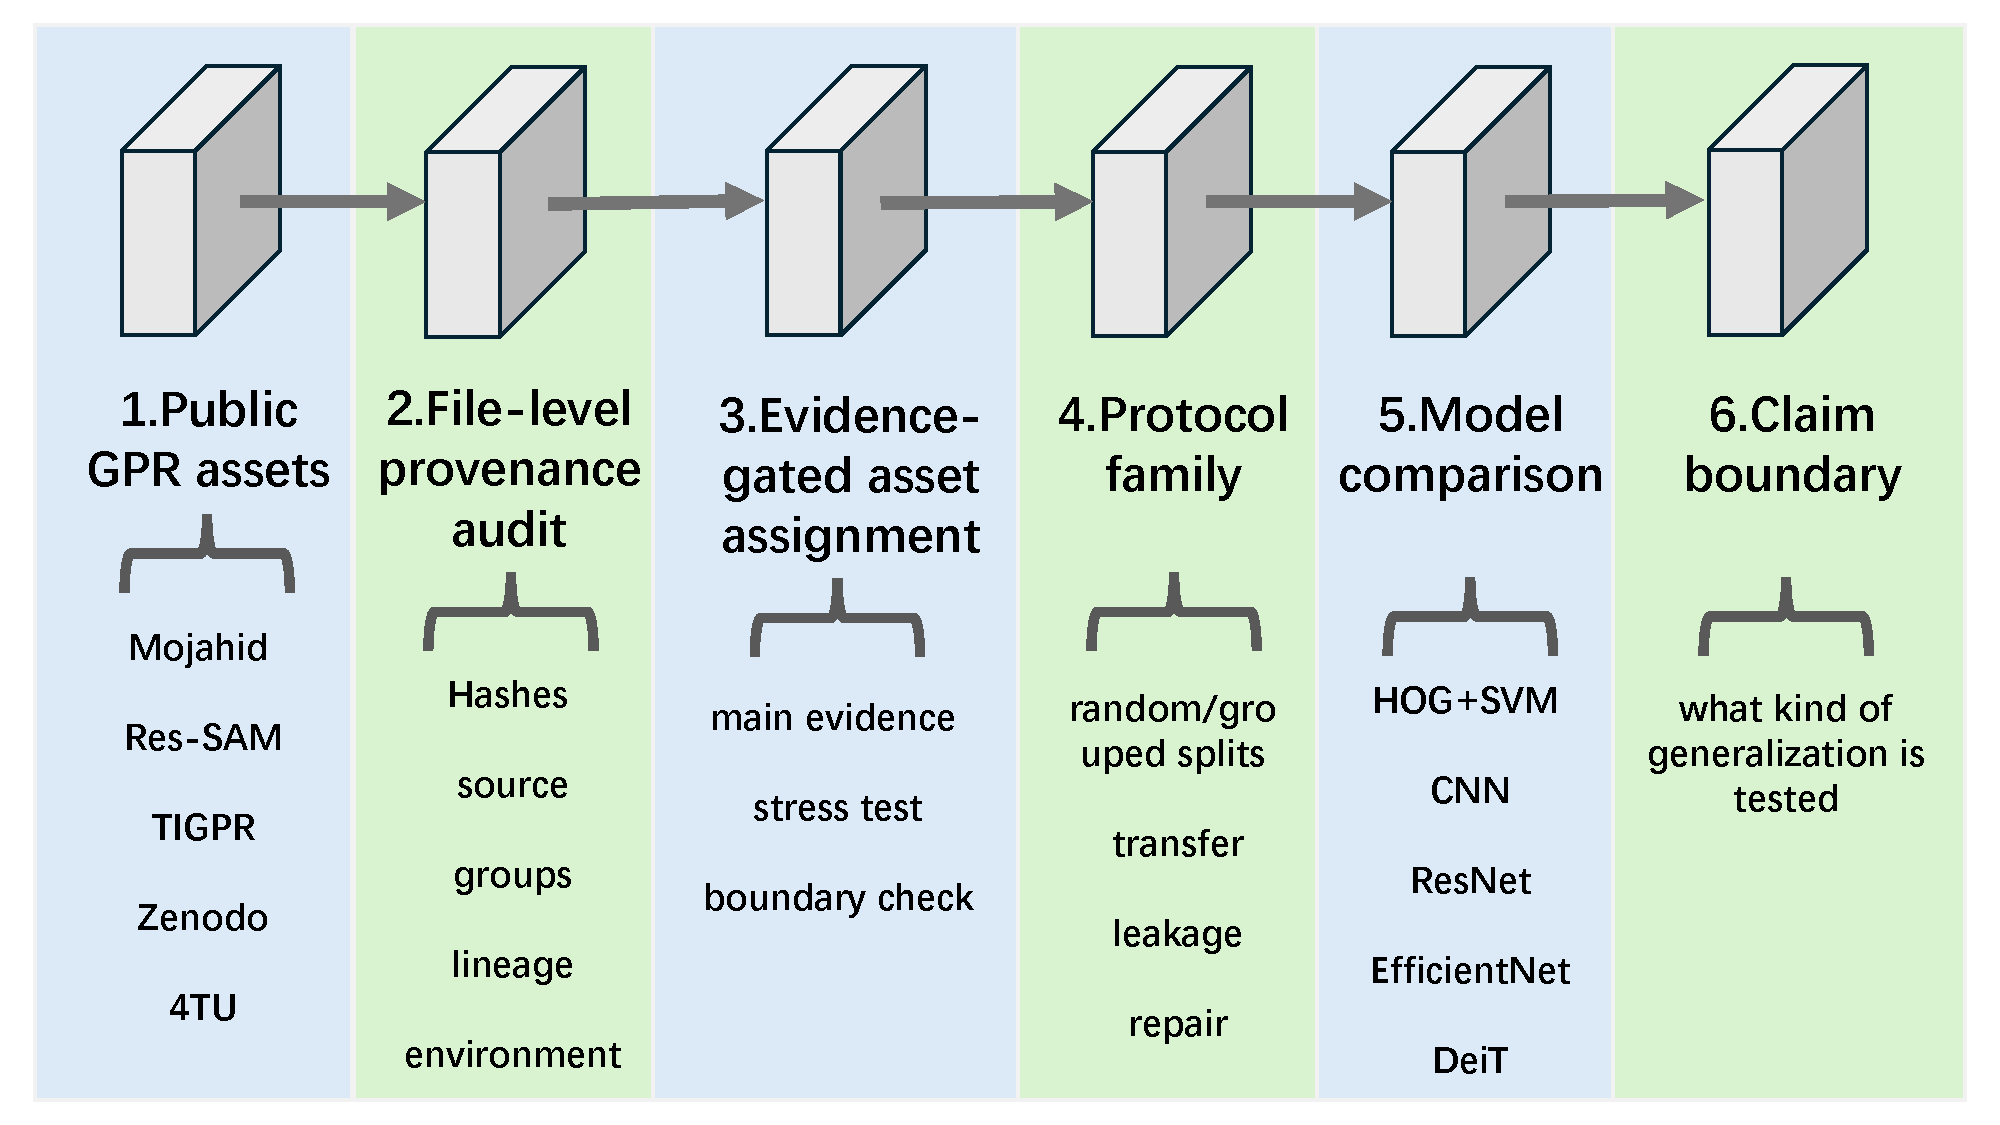
\includegraphics[width=\textwidth]{fig1_workflow.pdf}
\caption{Study design and evidence gates. The workflow separates the local asset audit, split and transfer baselines, raw-trace stress tests, blind external protocol and manuscript claim boundary before interpreting model performance.}
\label{fig:workflow}
\end{figure}

\begin{table}[H]
\caption{Dataset and provenance inventory used to assign each public asset to an evaluation role.}
\label{tab:asset_inventory}
\centering
\footnotesize
\setlength{\tabcolsep}{4pt}
\renewcommand{\arraystretch}{1.08}
\begin{tabular}{L{0.15\textwidth}L{0.10\textwidth}L{0.34\textwidth}L{0.31\textwidth}}
\toprule
Asset & Rows & Evaluation use & Boundary for interpretation \\
\midrule
Mojahid & 2,524 & executable grouped-split and augmentation-lineage analysis & single-source exploratory asset; not sufficient alone for confirmation \\
Res-SAM & 1,050 & executable acquisition-environment transfer and model matrix & not an independent external asset \\
4TU & 99 & executable raw-trace perturbation stress test & project count and metadata balance limit main-confirmation use \\
TIGPR & 7,169 & supporting duplicate-aware provenance evidence & verified local index not used as core evidence \\
Zenodo 14637589 & 914 & supporting raw-file source-group split stress test & image-level semantics limited by the available manifest \\
DeepMask & 2,524 & linked derivative for augmentation and hash-lineage audit & hashes match Mojahid and are not independent confirmation \\
\bottomrule
\end{tabular}
\end{table}

Each manifest recorded the dataset, sample identifier, task label, label source, file path, SHA-256 digest, dimensions and export format. Project, activity, site, survey line, device, acquisition setting and processing chain were added when available. The protocol fields recorded source group, fold, augmentation status, augmentation ancestor and exact-duplicate group. Model analyses used readable files with a sample identifier, task label and the grouping field required by the protocol. Raw-trace labels were joined through activity-level records. Equal SHA-256 hashes defined exact duplicates. Perceptual hashes and pairwise Hamming distances were also calculated to identify image-equivalent exports with different byte hashes.

The manifest was built before model fitting. This ordering avoided assigning groups after a model result was known. For each sample, the hash was calculated from the local file actually used by the experiment. The manifest also recorded whether an image came from an original file, an augmented derivative, a rendered export or a raw-trace-derived matrix. When a required field was missing, the asset was still retained if it could support another analysis, but it was not used for a protocol that required that missing field. For instance, a dataset without a recoverable environment label could not contribute to bidirectional environment transfer, whereas it could still contribute to duplicate or random-versus-grouped split analysis. This rule kept the protocol executable across heterogeneous public releases.

\subsection{Provenance structure}

Three classification tasks measured the source information carried by the images: Mojahid processing role, Mojahid augmentation lineage and Res-SAM acquisition environment. Images were converted to grayscale, resized to $64\times64$ pixels and scaled to $[0,1]$. Histograms of oriented gradients (HOG) used $8\times8$ pixel cells, nine unsigned orientation bins and cell-wise $L_2$ normalization. The standardized features were fitted with SGD logistic regression using $\alpha=10^{-4}$, balanced class weights and a maximum of 1,000 iterations. Lineages represented by fewer than eight images were omitted from the lineage task. Each task used five 70:30 stratified train--test splits with seeds 20260811--20260815. Res-SAM splits were stratified jointly by class and environment where the sample counts allowed.

Associations between task labels and source groups were summarized by normalized mutual information, Cramer's $V$ and group purity. Cramer's $V$ was calculated from the label-by-source contingency table, and purity was averaged across source groups without weighting by group size. Significance was assessed from 1,000 permutations of the source labels using seed 20260811. The permutation $p$ value was $(b+1)/1,001$, where $b$ denotes the number of permuted mutual-information values at least as large as the observed value.

The source-prediction tasks were diagnostic rather than performance baselines. Their purpose was to test whether a simple representation could recover information about processing role, lineage or environment from the same files used for recognition. High source predictability did not by itself prove that a recognition model used source information. It showed that source information was available to a learner and therefore needed to be controlled by the split design. The association statistics answered a second question: whether the source variables were also aligned with the target labels. When both conditions were present, random splitting could mix class evidence with source structure, and grouped or transfer tests became necessary.

The three diagnostics were read together. Source prediction measured feature-level recoverability. Normalized mutual information measured how much label information was shared with the source variable. Group purity measured whether individual source groups were nearly class-specific. This combination was chosen because no single statistic captured the whole risk. A source variable can be predictable without being label-aligned, or label-aligned without being easy to recover from pixels. The benchmark treated the risk as strongest when source information was recoverable from the files and was also associated with the class labels.

\subsection{Models and image preprocessing}

Five model families were compared on Mojahid and Res-SAM. The first combined HOG features with a training-set StandardScaler and an RBF-SVM ($C=3$, \texttt{gamma=scale}, balanced class weights). The lightweight CNN received $64\times64$ grayscale images and comprised three $3\times3$ convolutional blocks with 8, 16 and 32 channels, batch normalization and ReLU activations. The first two blocks used $2\times2$ max pooling, and the third used adaptive $4\times4$ pooling. The classifier contained a 64-unit fully connected layer, dropout of 0.20 and a linear output layer. It was trained for eight epochs with class-weighted cross-entropy and AdamW (learning rate $10^{-3}$, weight decay $10^{-3}$, batch size 64).

ResNet18, EfficientNetB0 and DeiT-Tiny supplied frozen ImageNet features. Their RGB inputs were resized bilinearly to $128\times128$, $128\times128$ and $224\times224$ pixels, respectively, and normalized with the ImageNet channel statistics. The three feature vectors had 512, 1,280 and 192 dimensions. Standardized embeddings were classified with LinearSVC ($C=1$, balanced class weights, 30,000 maximum iterations). The five families used seeds 20260810--20260814 and the same family-specific hyperparameters in every protocol.

The model set was chosen to cover common levels of recognition complexity without turning the paper into an architecture search. HOG+RBF-SVM represented a strong hand-crafted baseline for structured B-scan images, combining oriented-gradient descriptors and support-vector classification \cite{dalal2005hog,cortes1995svm}. The lightweight CNN tested whether a small trainable network changed the split effect when trained directly on the benchmark images. ResNet18 and EfficientNetB0 represented convolutional ImageNet features at two capacities, and DeiT-Tiny represented a compact transformer feature extractor \cite{deng2009imagenet,he2016resnet,tan2019efficientnet,touvron2021deit}. Keeping the deep models frozen made the comparison less dependent on small-dataset fine-tuning noise and made the split protocol the main variable. All model families were evaluated under the same train--test definitions for a given asset.

Preprocessing was deliberately simple. Images were resized and normalized in a way that preserved the visible B-scan structure while allowing the five model families to receive consistent inputs. No target-set statistics were used in the non-transductive baseline. For HOG and pixel models, the scaler was fitted on the training split only and then applied to validation and test splits. For frozen deep features, ImageNet normalization was fixed before feature extraction. These choices reduced the number of places where train--test information could enter through preprocessing, which was important because the study focused on provenance and split effects rather than on maximizing absolute recognition accuracy.

\subsection{Partitioning, transfer and stress tests}

For Mojahid, stratified random 80:20 partitions were compared with the supplied lineage-aware folds. Fold 0 served as the grouped test set, fold 1 was set aside, and the remaining folds formed the training set. Random partitions were regenerated for each seed; the grouped test set was fixed. Res-SAM within-environment models used separate stratified 80:20 partitions for the real and synthetic subsets. Bidirectional transfer used the shared cavity, crack and pipe classes, training on one environment and testing on the other. Transfer loss was the difference between target-environment within-set balanced accuracy and transfer balanced accuracy.

The unified split analysis covered Mojahid, TIGPR, Zenodo and DeepMask. The random reference assigned 70\%, 15\% and 15\% of each class to training, validation and test sets by a deterministic hash with seed 20260811. Grouped protocols kept each source group in a single partition. Source-group holdout targeted 70:15:15 sample proportions. Provenance-size holdout assigned the largest class-specific groups first and targeted 70:10:20. Existing dataset folds were used where available; otherwise, a 70:10:20 grouped partition was generated. A deterministic group-balance assignment formed the fifth condition. Image assets were represented by standardized HOG features, while the Zenodo files used file size and head--tail byte signatures. SGD logistic regression supplied the split comparisons. Model-ranking comparisons added ExtraTrees with 160 trees and a minimum leaf size of two.

The random reference was retained because it is the most common baseline in image-recognition papers and gives the reader a familiar point of comparison. The grouped protocols were designed to ask a different question. Instead of asking whether a model recognizes examples drawn independently from the pooled asset, they ask whether performance remains when related files are kept together. Source-group holdout tests whether entire groups can be withheld. Provenance-size holdout makes the test stricter by assigning large groups first, which reduces the chance that a dominant source group is split across partitions. Existing folds were used when a dataset already supplied them, because those folds represent the data provider's intended evaluation. Deterministic group balance then tested whether a reproducible group assignment with class balancing gave the same conclusion.

The Res-SAM transfer protocol separated within-environment recognition from cross-environment generalization. Within-environment splits tested whether a model could classify held-out samples from the same environment pool. Synthetic-to-real and real-to-synthetic transfer tested whether the same learned decision rule carried across the environment boundary. The transfer classes were restricted to cavity, crack and pipe because these labels appeared in both environments. This restriction avoided comparing scores across different label spaces. Transfer loss was calculated relative to the target environment's own within-set result, so that each transfer direction was judged against the performance that was achievable inside the environment being tested.

Duplicate experiments compared random partitions with partitions that kept related samples together. TIGPR duplicate groups were defined by SHA-256 and assigned with five-fold stratified group partitioning. Five random 80:20 splits were compared with hash-group-disjoint splits. For duplicate doses of 0, 0.05, 0.10, 0.20 and 0.40, one member of a selected same-label duplicate group was moved into training and another remained in testing. The Mojahid lineage-dose experiment used the same dose levels and split each selected test lineage equally between training and testing. DeepMask was evaluated with random 80:20 and base-source-group 80:20 partitions. Directional augmentation tests trained on augmented images and tested on originals, and then reversed the two roles, using HOG, downsampled pixels and metadata features.

The duplicate-dose design measured a controlled version of a common public-data problem. It did not assume that all duplicates are harmful. Instead, it asked how the test score changes when a known fraction of test examples has a same-label duplicate or close lineage member in the training set. The dose levels were selected to span small accidental leakage and larger systematic sharing. For Mojahid, lineages rather than exact byte duplicates were used because augmented derivatives can be visually related even when the hash differs. For TIGPR, byte-level duplicates were sufficient to construct a direct duplicate-sharing experiment. These two cases therefore tested related but distinct channels of non-independence.

The 4TU analysis applied seven transformations to each raw-trace matrix: signed log compression, clipped per-matrix standardization, amplitude contraction, upper-band removal, lower-band removal, border removal and time reversal. The matrices were rendered at $64\times64$ pixels before HOG extraction. ExtraTrees, RBF-SVM and a majority baseline were fitted to the original training matrices, and validation balanced accuracy selected the classifier used on the unchanged and transformed test sets. Fixed-fold experiments used five seeds. Each of five project-aware partitions used two validation and two test projects and retained all classes.

The perturbations were chosen to separate class recognition from simple sensitivity to rendering or matrix-level preprocessing. Signed log compression changed the amplitude scale while retaining sign information. Clipped standardization removed large per-matrix amplitude differences. Band removal tested whether upper or lower parts of the matrix carried disproportionate information. Border removal tested whether edge content contributed to the score. Time reversal served as a negative stress test because it preserves many marginal statistics while disrupting the physical order of the trace. The same trained classifier was evaluated on original and perturbed test matrices, so the measured delta reflected perturbation response rather than retraining.

Table~\ref{tab:evaluation_protocols} lists the protocol families and the claim tested by each partition or stress-test design.

\begin{table}[H]
\caption{Evaluation protocols used to separate within-asset recognition, grouped generalization, cross-environment transfer and stress-test evidence.}
\label{tab:evaluation_protocols}
\centering
\footnotesize
\begin{tabular}{p{0.19\textwidth}p{0.15\textwidth}p{0.24\textwidth}p{0.30\textwidth}}
\toprule
Protocol family & Main asset(s) & Primary contrast & Question answered \\
\midrule
Source diagnostics & Mojahid, Res-SAM & source predictability and label--source association & Are provenance variables recoverable and label-aligned before recognition? \\
Random versus grouped splits & Mojahid, TIGPR, Zenodo, DeepMask & random split minus group-disjoint split & Does sample grouping change within-asset recognition? \\
Environment transfer & Res-SAM & within-environment score minus cross-environment score & Does a learned decision rule carry across acquisition environments? \\
Duplicate or lineage dose & Mojahid, TIGPR & zero-dose split versus controlled related-sample sharing & Does related-sample sharing alter scores or class-level errors? \\
Raw-trace stress tests & 4TU & original matrices versus perturbed matrices & Does preprocessing or project structure affect raw-trace classifiers? \\
Repair controls & Mojahid, Res-SAM, 4TU & baseline versus train-only calibration, weighting, repair or alignment & Do simple controls remove the provenance effect? \\
\bottomrule
\end{tabular}
\end{table}

\subsection{Calibration and representation controls}

Mojahid temperature scaling used logits from HOG logistic regression. Temperature was selected by validation negative log likelihood from 91 values between 0.5 and 5.0 and applied to the test logits. Source reweighting compared uniform weights with inverse class-frequency, source-frequency and joint label--source weights, each normalized to a mean of one. Additional training-set controls removed one linear direction associated with processing role, selected HOG dimensions with a source-predictability penalty, and optimized Group-DRO objectives over source, label--source or processing-role groups. A gradient-reversal network used domain-adversarial weights of 0, 0.1, 0.5 and 1.0; validation target balanced accuracy selected the checkpoint.

Res-SAM preprocessing controls used per-image standardization clipped to $[-3,3]$ or rank-based histogram equalization before HOG extraction. Source-style augmentation pooled raw, standardized and equalized versions of the source training images. Transductive variants estimated HOG mean--variance alignment or CORAL covariance alignment from unlabeled target images, with CORAL regularization set to $10^{-3}$. The 4TU comparison included per-matrix standardization, target mean--variance alignment and CORAL.

The repair experiments were designed as controls, not as a search for a new adaptation method. They tested whether simple changes that are common in small image studies could explain away the provenance effect. Temperature scaling adjusted confidence without changing the predicted class \cite{guo2017calibration}. Source reweighting changed the importance of training examples but used only training-set labels and source groups. Direction removal, source-confusion feature selection and domain-adversarial training reduced explicit source predictability in the representation \cite{ganin2016domain}. Res-SAM and 4TU alignment variants then tested whether simple distribution matching could recover transfer performance \cite{sun2016coral}. A repair was considered informative only if it improved target balanced accuracy without using target labels.

\subsection{Statistical analysis and reproducibility}

Balanced accuracy, the unweighted mean of class recall, was the primary measure. Accuracy and macro-averaged F1 were secondary measures. Models with probabilistic outputs also reported ten-bin expected calibration error, negative log likelihood, mean confidence, class-specific recall, worst-class recall and recall spread. Seed results are given as the arithmetic mean and population standard deviation. In the five-family comparison, directional support was a positive within-minus-transfer or random-minus-grouped difference; a difference of at least 0.05 was considered material.

Confidence intervals for fixed unified-split contrasts used 2,000 class-stratified bootstrap samples from each test prediction set. The 2.5th and 97.5th percentiles formed the 95\% interval. One-sided bootstrap $p$ values used the add-one proportion of random-minus-protocol draws at or below zero. Aggregate directions were tested with an exact binomial sign test and exhaustive sign flips over dataset--protocol contrasts. The 4TU fixed-fold and project-aware log-compression analyses used 10,000 bootstrap draws and the same sign procedures. The inferential units were protocol or seed contrasts. Diagnostic $p$ values are reported without multiplicity adjustment.

Experiments ran in Python 3.12.5 with NumPy 2.1.3, scikit-learn 1.5.2, Pillow 12.2.0, PyTorch 2.8.0, torchvision 0.23.0 and timm 1.0.27. PyTorch and torchvision used CPU builds. Each run produced a dated JSON summary and CSV records containing the run identifier, manifest, protocol, model, seed and metrics. Split manifests recorded the assignment, source group and SHA-256 digest of every sample. A checkpoint script verified the manifests, software imports and expected outputs before source-data generation.

The statistical analysis emphasized repeated direction and effect size over a single omnibus test. This choice matched the study design. The assets differed in file type, class structure and available provenance fields, so their scores were not pooled as if they were repeated measurements of one identical task. Instead, each protocol produced a contrast, such as random minus grouped or within-environment minus transfer. The sign, magnitude and bootstrap interval of that contrast were then examined across assets and model families. This makes the summary robust to one dataset having larger sample count or easier labels than another. It also keeps the main claim tied to the experimental question: whether changing the provenance condition changes the interpretation of the score.

Reproducibility checks were run at the file and protocol levels. File checks verified that every listed path existed, that hashes matched the manifest and that each sample had the fields required by its assigned protocol. Split checks verified that group-disjoint protocols did not place the same source group in more than one partition. Duplicate checks verified that duplicate-aware partitions kept the same hash group together unless the experiment intentionally introduced a leakage dose. Run checks compared the expected number of rows, classes and seeds with the produced metric tables. These checks were included because a provenance benchmark can fail silently if a file is missing, a group field is changed or a split is regenerated with different identifiers.

The audit records were kept separate from the model outputs. This separation allowed a split or manifest problem to be detected before model performance was inspected. It also made the benchmark rerunnable when a new model family was added. For each protocol, the model consumed a fixed train, validation and test table rather than generating its own partitions internally. This rule was used for both classical and deep-feature models. It prevented implementation details inside a model wrapper from changing the evaluation question and made the split definition the stable reference point across experiments.

\section{Results}

\subsection{Public GPR assets contain recoverable source structure}

We first checked which files could be used in each analysis. The manifests contained 2,524 Mojahid images, 99 4TU matrices, 1,050 Res-SAM images, 7,169 TIGPR images and 914 Zenodo raw files. DeepMask added 2,524 rows with file hashes identical to Mojahid and was used to track augmentation lineages. This file-level accounting set the scope for grouped evaluation, cross-environment transfer, duplicate analysis and raw-trace stress testing.

Source information could be recovered from the images. Res-SAM environment prediction reached balanced accuracy 0.9926 against a 0.5 chance level. Mojahid processing-role prediction reached balanced accuracy 0.6010, and the 80-class Mojahid source-group task reached 0.6079 against a 0.0125 chance baseline. The corresponding accuracies were 0.6319, 0.6006 and 0.9930, and the macro-F1 values were 0.5877, 0.5995 and 0.9929. Thus, acquisition environment, processing role and lineage were present in the image records before class recognition was evaluated.

The same source variables were associated with labels. In Mojahid, label versus source-group association had NMI 0.2514, Cramer's V 0.8724, a mutual-information test p value of 0.0010, mean source purity 0.9796 and pure source groups covering 0.9465 of groups. Label versus processing role also had measurable association, with NMI 0.1079, Cramer's V 0.4265, p = 0.0010 and mean source purity 0.5749. In Res-SAM, label versus environment association had NMI 0.1699, Cramer's V 0.5477, p = 0.0010 and mean source purity 0.2500. Provenance acted as both a file-level descriptor and a label-organisation variable in these assets.

These diagnostics were important because they were run before the recognition comparisons. They showed that the benchmark files already contained non-class structure that a simple learner could recover. The Mojahid source-group result was not a small deviation from chance: the 80-class task reached 0.6079 balanced accuracy, far above the 0.0125 chance level. Res-SAM environment prediction was close to perfect, which meant that real and synthetic exports were visually or statistically separable in the benchmark representation. The association tests then showed that the same source variables were not independent of class labels. This combination gave a concrete reason to treat random splits as a weak reliability test rather than as the default answer.

The purity values also explained why grouped tests were needed even when the nominal class labels looked balanced. In Mojahid, most source groups were nearly pure with respect to class. A random split can therefore place related samples from a nearly class-specific source group into both training and test partitions. Under that condition, a classifier can partly learn group-specific regularities and still appear to perform a class-recognition task. The grouped protocols removed that shortcut by assigning the whole group to one partition. In Res-SAM, the environment association was weaker by purity but stronger by direct environment predictability, which made environment transfer the more appropriate test than lineage holdout.

\subsection{Cross-environment testing separates within-set and transfer performance}

The largest separation appeared when Res-SAM models were moved between real-world and synthetic samples. In the HOG+RBF-SVM seed sweep, balanced accuracy was 0.8483 \(\pm\) 0.0308 within real-world data and 0.9067 \(\pm\) 0.0279 within synthetic data. Training on synthetic samples and testing on real-world samples gave balanced accuracy 0.4367. Training on real-world samples and testing on synthetic samples gave 0.3511. The within-minus-transfer differences were 0.4116 and 0.5556.

Table~\ref{tab:main_results} gives the main numerical contrasts used in the Results narrative. Figure~\ref{fig:cross_model_transfer} summarizes the five-family contrasts and shows why Res-SAM transfer is the strongest current cross-model result.

\begin{table}[H]
\caption{Primary numerical contrasts used to interpret the benchmark results.}
\label{tab:main_results}
\centering
\footnotesize
\begin{tabular}{p{0.20\textwidth}p{0.24\textwidth}p{0.20\textwidth}p{0.24\textwidth}}
\toprule
Asset and protocol & Model or contrast & Balanced accuracy & Interpretation \\
\midrule
Res-SAM real-world within-set & HOG+RBF-SVM & \(0.8483 \pm 0.0308\) & target-environment baseline for synthetic-to-real transfer \\
Res-SAM synthetic-to-real & HOG+RBF-SVM & 0.4367 & large cross-environment loss \\
Res-SAM synthetic within-set & HOG+RBF-SVM & \(0.9067 \pm 0.0279\) & target-environment baseline for real-to-synthetic transfer \\
Res-SAM real-to-synthetic & HOG+RBF-SVM & 0.3511 & largest transfer loss in the seed sweep \\
Mojahid random split & HOG+RBF-SVM & \(0.9543 \pm 0.0049\) & higher score when related lineages can share partitions \\
Mojahid grouped split & HOG+RBF-SVM & \(0.8566 \pm 0.0000\) & lower score under lineage-aware testing \\
4TU log-clip perturbation & ExtraTrees HOG fixed split & \(0.0905 \pm 0.0095\) & raw-trace stress-test signal, not main confirmation evidence \\
\bottomrule
\end{tabular}
\end{table}

\begin{figure}[H]
\centering
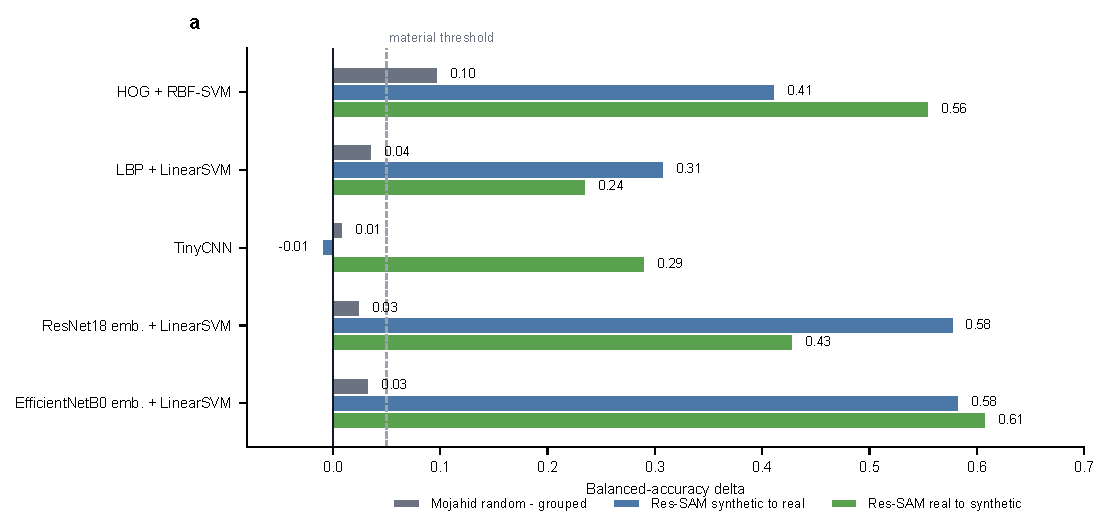
\includegraphics[width=\textwidth]{fig2_cross_model_transfer.pdf}
\caption{Cross-model evidence for provenance effects. The five model families show a consistently positive within-minus-transfer contrast for Res-SAM, while the Mojahid random-minus-grouped contrast is smaller but remains positive across the same family set.}
\label{fig:cross_model_transfer}
\end{figure}

The multi-model synthesis gave the same ordering. For real-to-synthetic transfer, all five model families had a material positive within-minus-transfer contrast, with a mean balanced-accuracy delta of 0.4888. For synthetic-to-real transfer, four of five families met the material threshold, with a mean delta of 0.4139. The five families were HOG+RBF-SVM, lightweight CNN, ResNet18, EfficientNetB0 and DeiT-Tiny, covering both hand-crafted features and frozen deep representations.

The bidirectional design helped separate two possible explanations. If the effect had appeared only for one model family, it could have been attributed to a particular representation. If it had appeared only for one direction, it could have been read as a peculiarity of either the real-world or synthetic subset. Instead, the transfer gap was present across hand-crafted HOG features, a small trainable CNN and three frozen deep feature extractors, and it appeared in both transfer directions. The exact values differed by model family, but the ordering stayed the same: within-environment evaluation gave much higher balanced accuracy than testing on the other acquisition environment.

This result also changed how the high within-environment scores should be read. The real-world and synthetic subsets were both learnable when training and testing stayed inside the same environment. That means the low transfer scores were not simply a failure of the classes to be separable. They showed that the decision boundary learned from one environment did not carry cleanly to the other. For a GPR recognition benchmark, this is the more relevant reliability signal. A model can look useful under an internal split and still be uncertain when the acquisition source changes.

\subsection{Split choice changes rankings and scores}

Changing the split changed both the score and the top-ranked model. On Mojahid, SGD logistic regression led under random stratified and existing-fold splits. ExtraTrees led under source-group holdout, provenance-size holdout and deterministic group balance. In the HOG+RBF-SVM five-seed experiment, random-split balanced accuracy averaged 0.9543, grouped-split balanced accuracy averaged 0.8566 and the random-minus-grouped delta was 0.0976. In the five-family synthesis, the Mojahid random-minus-grouped contrast stayed positive for all five families, with a mean delta of 0.0371.

Figure~\ref{fig:mojahid_split} separates the Mojahid seed sweep from the five-family model comparison and shows that the grouped-split result changes both score level and ranking.

\begin{figure}[H]
\centering
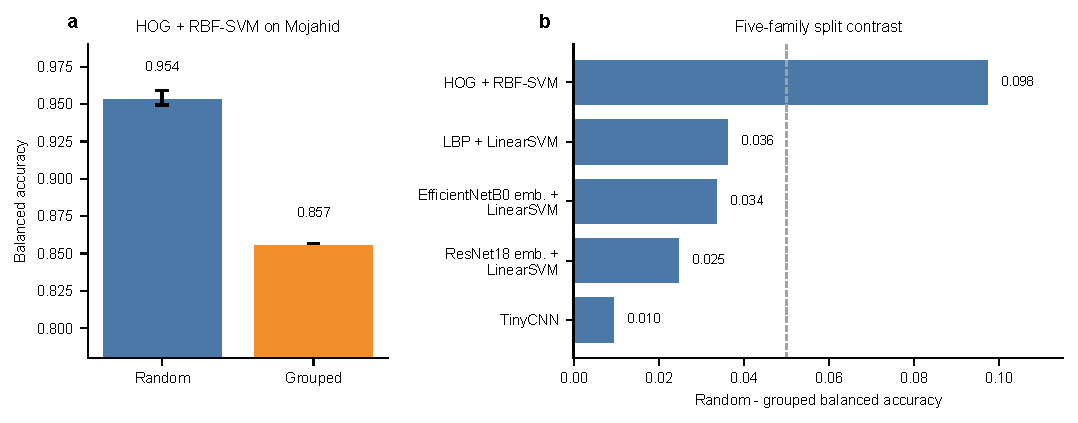
\includegraphics[width=\textwidth]{fig3_mojahid_split.pdf}
\caption{Mojahid split sensitivity. The HOG+RBF-SVM seed sweep shows a stable random-minus-grouped difference, and the five-family comparison shows that the sign of the split effect remains positive while the preferred model changes with the partition rule.}
\label{fig:mojahid_split}
\end{figure}

The unified split analysis was positive for most asset-protocol contrasts. For Mojahid, random-minus-existing-fold was +0.0826 with a 95\% bootstrap interval of [0.0290, 0.1357] and p = 0.0030. Random-minus-source-group-holdout was +0.1219 [0.0532, 0.1863], p = 0.0010; random-minus-provenance-size-holdout was +0.1670 [0.1064, 0.2280], p = 0.0005; and random-minus-deterministic-group-balance was +0.1219 [0.0568, 0.1871], p = 0.0005. Across the 16 unified split contrasts, 15 were positive and the exact sign test gave p = 0.0003. The sign-flip audit gave the same direction.

The size of the split effect was asset specific. TIGPR had an existing-fold delta of \(-0.0073\) [-0.0530, 0.0353], p = 0.6387, and a source-group-holdout delta of +0.0128 [-0.0371, 0.0594], p = 0.3098. Its provenance-size-holdout contrast was +0.0516 [0.0065, 0.0956], p = 0.0110. Zenodo showed its strongest change under provenance-size holdout, +0.3055 [+0.2294, +0.3776], p = 0.0005. DeepMask was positive across all four contrasts, with deltas from +0.1124 to +0.1188 and p = 0.0005. In the IOAI Radar split-stress audit, the official train-to-validation and train-to-test partitions gave balanced accuracies of 0.5466 and 0.5305 for the tertile task; random stratified splits ranged from 0.51 to 0.54.

The asset-specific pattern is useful because it prevents a single over-generalized conclusion. TIGPR did not show a large penalty under every grouped protocol, but its provenance-size holdout did produce a positive contrast. Mojahid and DeepMask showed clearer split sensitivity, consistent with the recovered lineage and base-source structure. Zenodo gave the largest provenance-size-holdout effect, which fits a raw-file asset where source grouping can dominate a simple file-signature baseline. IOAI did not produce a strong random-split advantage in the available tertile task and was therefore read as a split-stress audit rather than as main evidence for the paper. The point is not that every public GPR asset fails the same way. The point is that the split condition changes what the score means.

The model-ranking changes made the same point from another angle. If only the absolute score changed, one might treat grouped splitting as a stricter but otherwise equivalent version of random splitting. Instead, the leading model changed across protocols. On Mojahid, SGD logistic regression led under random stratification and existing folds, whereas ExtraTrees led under source-group, provenance-size and deterministic group-balance holdouts. This matters for benchmark reporting because leaderboards are often used to choose a model family. A ranking derived from random splits may select a different model than a ranking derived from source-separated evaluation.

\subsection{Seed repeats retain the split effect}

The split differences were stable across repeated seeds. In the unified split seed-stability sweep with five SGD-logistic seeds, Mojahid balanced accuracy was 0.8373 \(\pm\) 0.0106 under random stratification, 0.7607 \(\pm\) 0.0140 under existing folds, 0.7283 \(\pm\) 0.0177 under source-group holdout and 0.6902 \(\pm\) 0.0137 under provenance-size holdout. Zenodo followed the same direction, with 0.8941 \(\pm\) 0.0053 under random stratification and 0.6145 \(\pm\) 0.0189 under provenance-size holdout. Using the random-minus-protocol contrast as the inferential unit, 15 of 16 all-asset contrasts were positive.

The seed sweep reduced the chance that the split effect was caused by one favourable partition. The standard deviations were small relative to the random-minus-grouped differences, especially for Mojahid and Zenodo. For Mojahid, the average gap from random stratification to provenance-size holdout was about 0.1471 balanced-accuracy points, while the seed standard deviations were around 0.01--0.02. For Zenodo, the random to provenance-size gap was about 0.2796. These magnitudes were much larger than the seed-to-seed variation. The conclusion therefore did not depend on a single lucky or unlucky seed.

This stability is important for a benchmark paper because random seeds are often treated as an implementation detail. In these experiments, the seed was not the main source of uncertainty. The choice of partitioning rule had the larger effect. Reporting mean and standard deviation over random splits is still useful, but it does not replace a grouped or provenance-aware split when related samples exist. A stable random-split result can be stable for the wrong evaluation question.

\subsection{Leakage and duplicates affect class-level errors}

Controlled leakage changed the mean score and the class-level error profile. In the Mojahid lineage leakage-dose sweep, balanced accuracy increased from 0.8566 at dose 0.00 to 0.8983 at dose 0.40. Worst-class recall rose from 0.6905 to 0.7666, while recall spread narrowed from 0.2996 to 0.2181. Calibration metrics moved as well: ECE decreased from 0.0365 to 0.0230 and mean confidence increased from 0.9015 to 0.9155.

Duplicate and augmentation structure produced additional random-split effects. TIGPR contained 7,169 samples, 243 duplicate groups, 486 duplicate images and two cross-label duplicate groups. In the duplicate-aware baseline, hash-group splitting gave HOG balanced accuracy 0.6777, whereas random splitting reached 0.7314 and shared 76.6 duplicate hash groups on average. The metadata baseline moved from 0.8892 to 0.8847. A restored duplicate-leakage dose experiment increased balanced accuracy from 0.6777 at zero dose to 0.6898 at dose 0.20. DeepMask showed a related augmentation effect: its 2,524 rows traced to 285 base source groups, and the best random split exceeded the best group-holdout split by 0.0407. A TIGPR file-level perceptual-hash sweep found 246 pHash collision groups covering 492 images. Three collision groups spanned distinct file-hash groups, and those pairs were same-label, zero-Hamming matches.

The class-level changes show why leakage should not be summarized only by the average score. In the Mojahid lineage-dose experiment, the worst-class recall improved as more lineage sharing was introduced. This made the model look more balanced across classes, not just more accurate on average. At the same time, calibration appeared to improve because ECE decreased and mean confidence increased. Those changes are plausible outputs of a test set that has become more familiar to the model. They are also difficult to detect from accuracy alone. A leakage-aware benchmark therefore needs class recall and calibration summaries in addition to the primary balanced-accuracy score.

The duplicate findings also showed that exact byte hashes are necessary but not sufficient. TIGPR contained exact duplicate groups that could be assigned together by hash. The pHash sweep then found visually identical or near-identical exports that did not always share the same byte-level grouping. This matters for public image datasets because re-saving, resizing or metadata changes can alter the file hash while preserving the visible signal. The benchmark used SHA-256 as the strict duplicate definition and pHash as an additional audit. The two checks serve different purposes: SHA-256 gives a reproducible equality test, while pHash flags image-equivalent files that may deserve grouped handling.

The directional augmentation tests were included because augmentation is not symmetric. Training on augmented images and testing on originals asks whether augmented derivatives contain enough class information to recover the original distribution. Training on originals and testing on augmented images asks whether the model is robust to the transformations used by the dataset. When both directions are mixed in a random split, the reported score can hide this distinction. DeepMask and Mojahid made this issue visible because their files shared a common lineage. In such cases, the benchmark should say whether augmentation is part of training only, testing only, or both sides of the split.

\subsection{Stress tests and repairs retain the provenance effect}

The 4TU raw-trace experiments tested the same question at the matrix level. In the Land type ExtraTrees fixed-split sweep, log-clip perturbation reduced mean balanced accuracy by 0.3429 and produced a mean flip rate of 0.8583, with exact sign and sign-flip p values of 0.0010. Under group-aware repeated splits, the mean delta decreased to 0.0422 in magnitude and the mean flip rate to 0.4693, with sign and sign-flip p values of 0.2500. A five-layer extension used summary features, raw pixels, HOG, a small CNN and group-aware HOG, placing 4TU as a stress test for preprocessing and project structure.

Figure~\ref{fig:stress_repair} and Table~\ref{tab:repair_controls} summarize the stress-test and repair evidence. The figure keeps the raw-trace perturbation signal separate from the grouped-split reduction, while the table records which train-only controls changed calibration, score or transfer.

\begin{figure}[H]
\centering
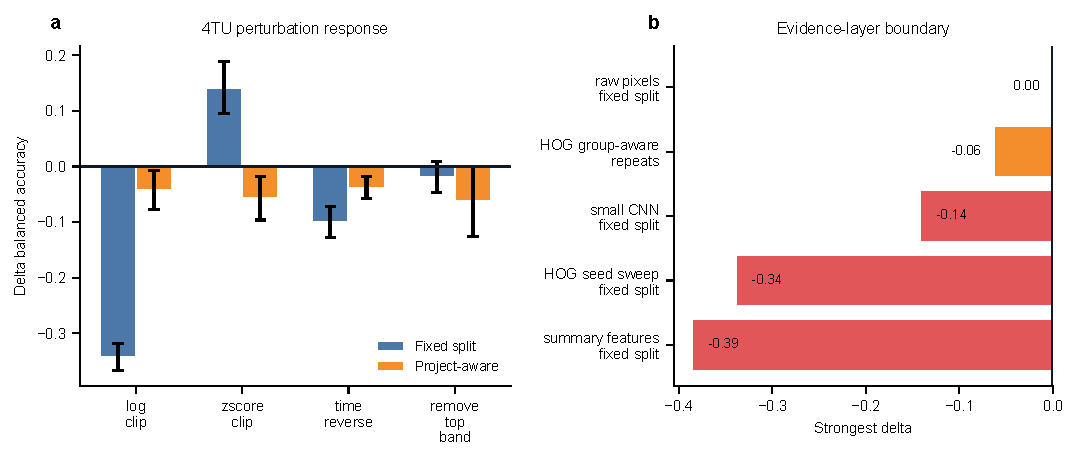
\includegraphics[width=\textwidth]{fig4_4tu_stress.pdf}
\caption{4TU raw-trace stress tests and train-only controls. The fixed-split perturbation has a large effect on balanced accuracy and prediction flips, while group-aware repeats reduce the magnitude. Simple alignment controls produce partial and protocol-dependent changes.}
\label{fig:stress_repair}
\end{figure}

\begin{table}[H]
\caption{Repair and calibration controls used to test whether the provenance effect could be removed by simple train-only adjustments.}
\label{tab:repair_controls}
\centering
\scriptsize
\setlength{\tabcolsep}{4pt}
\renewcommand{\arraystretch}{1.08}
\begin{tabular}{L{0.23\textwidth}L{0.27\textwidth}L{0.25\textwidth}L{0.15\textwidth}}
\toprule
Control & Baseline & Result after control & Interpretation \\
\midrule
Mojahid temperature scaling 1 & ECE 0.1651; BA 0.7741 & ECE 0.0296; BA unchanged & confidence only \\
Mojahid temperature scaling 2 & ECE 0.1208; BA 0.8210 & ECE 0.0297; BA unchanged & confidence only \\
Mojahid source reweighting & uniform weights & best BA delta 0.0000 & no gain \\
Mojahid source-direction removal & BA 0.7741 and 0.8210 & BA 0.6876 and 0.6807 & score fell \\
Res-SAM source-style augmentation & BA 0.4367 and 0.3511 & BA 0.4267 and 0.3400 & no recovery \\
4TU internal alignment control & raw BA 0.3857 & z-score 0.3714; mean--std 0.2762; CORAL 0.3429 & mixed response \\
\bottomrule
\end{tabular}
\end{table}

Calibration changed confidence estimates. On Mojahid, temperature scaling reduced ECE from 0.1651 to 0.0296 on one grouped protocol and from 0.1208 to 0.0297 on another, with balanced accuracy at 0.7741 and 0.8210. Source reweighting matched the uniform baseline in the audited protocols, with best balanced-accuracy delta 0.0000. Group-DRO objectives over source groups and label-source groups lowered balanced accuracy on the current protocol, while processing-role DRO gave gains of +0.0018 to +0.0025. Removing one source-discriminative HOG direction reduced target balanced accuracy from 0.7741 to 0.6876 and from 0.8210 to 0.6807, with source-probe balanced accuracy at chance. Domain-adversarial training reduced domain predictability, and source-confusion feature selection left the target score unchanged.

Repairs gave similar results in the transfer and raw-trace settings. On Res-SAM, source-style augmentation reached 0.4267 and 0.3400, compared with raw transfer baselines of 0.4367 and 0.3511. On 4TU Land type, non-transductive per-matrix z-score repair changed balanced accuracy from 0.3857 to 0.3714, while unlabeled-target mean/std and CORAL variants reached 0.2762 and 0.3429. Non-transductive preprocessing repair produced best deltas of +0.0033, +0.0000 and -0.0133 depending on protocol, and covariance alignment gave partial transfer recovery. The provenance effect remained after calibration, source weighting, representation repair and simple alignment.

The repair experiments narrowed the interpretation of the main effect. Temperature scaling improved calibration but left the class decisions unchanged, so it could not remove a transfer or grouped-split gap. Source reweighting and Group-DRO changed the training objective, but they did not produce a consistent improvement in the audited protocols. Removing a source-discriminative HOG direction reduced source predictability, yet it also reduced target balanced accuracy. This indicates that some source-correlated directions may also carry class-relevant signal. Simply erasing source information is therefore not a reliable repair for GPR recognition.

The Res-SAM and 4TU alignment controls reached the same conclusion from different data types. Source-style augmentation did not recover the Res-SAM cross-environment transfer scores. Mean--variance and CORAL alignment gave partial or inconsistent changes on 4TU and Res-SAM, depending on the protocol. These repairs were intentionally simple, but their outcome is informative. The observed provenance effect was not just a calibration artifact, a source-weighting artifact or a removable first-order distribution mismatch. For this benchmark, the safer interpretation is that provenance-aware evaluation exposes a real difference between within-source recognition and source-separated generalization.

The repair results also help position the benchmark for future method development. A new adaptation method can be added to the same split manifests and judged against the same within-environment, transfer and grouped-holdout contrasts. If the method improves only the random split, it has not addressed the provenance problem. If it improves transfer while retaining within-environment performance, it can be read as a genuine generalization gain. This makes the benchmark useful beyond the present model set.

\section{Discussion}

\subsection{Principal finding}

GPR-ProvenanceBench shows that measured generalization in GPR recognition depends on where the samples come from and how they are related. Res-SAM gives the clearest example: within-environment scores and cross-environment scores separated across several model families. Mojahid, DeepMask, TIGPR, Zenodo and 4TU point to the same issue from other parts of the workflow, including grouped splits, augmentation lineage, duplicate structure, seed repeats and raw-trace stress tests. The common message is simple: GPR benchmark scores are easier to interpret when sample history is reported before models are ranked.

The result is not a rejection of existing GPR recognition work. It is a change in what a reported benchmark score is asked to prove. A random split can be a useful internal development test, and it can show whether a representation contains class information. It cannot, by itself, show that the same decision rule will work across acquisition environments, source groups or duplicated lineages. GPR-ProvenanceBench makes that distinction visible by putting random, grouped, transfer and stress-test results next to each other. The strongest evidence comes from Res-SAM transfer, but the same evaluation logic applies to the other assets.

\subsection{Provenance-aware validation for GPR recognition}

This study makes provenance part of the validation record. We record file hashes, augmentation lineage, source groups, environment labels, duplicate structure and preprocessing controls before fitting or comparing models. That record separates questions that are often collapsed into one accuracy number: within-asset recognition, transfer between acquisition environments, random sharing of related samples, and the effect of calibration or repair. Because the workflow starts from files and split manifests, it can be applied to other public GPR collections without changing the recognition model.

Figure~\ref{fig:fourtu_feasibility} shows why the 4TU component is used as a stress-test and feasibility-boundary asset rather than as a main cross-model confirmation layer.

\begin{figure}[H]
\centering
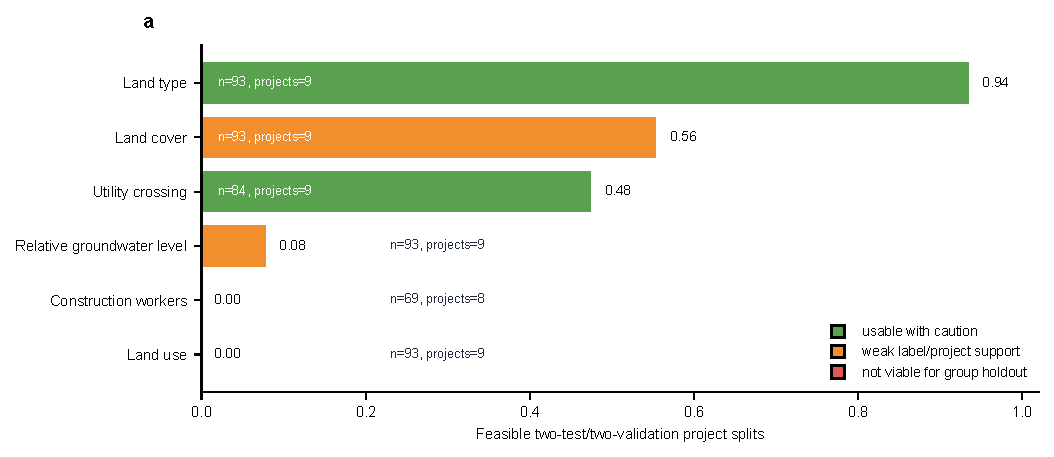
\includegraphics[width=\textwidth]{fig5_4tu_feasibility.pdf}
\caption{4TU feasibility boundary. The matrix count is low relative to the ten-project structure, and each Land type has limited project support. This evidence supports raw-trace stress testing and benchmark-boundary reporting rather than a standalone confirmation claim.}
\label{fig:fourtu_feasibility}
\end{figure}

This order is practical for NTE-style studies because it does not require a new sensing system or a new learning architecture. The same model can be evaluated under a stronger record of where each sample came from. For a road, bridge or subsurface inspection dataset, the source group might be a project, survey line, pavement section, specimen, antenna setting or rendering batch. For a public image dataset, it might be a base file, augmentation lineage or duplicate group. The exact grouping variable can differ across applications, but the reporting principle remains the same. The paper should state which relationships were kept apart and which relationships could not be reconstructed.

The workflow also gives a way to use imperfect public datasets without pretending that every file supports the same claim. Some assets support environment transfer, some support duplicate analysis and some support only stress testing. This is common in NDE data sharing because public releases are assembled for different purposes. A provenance-aware benchmark can still learn from those releases if it assigns each asset to the protocol it can actually support. That is more informative than discarding every incomplete asset or, conversely, treating every public file as an independent sample.

\subsection{Relationship to task-specific GPR studies}

Recent GPR studies in nondestructive evaluation usually start from a specific inspection task, such as runway compaction, bridge inspection, asphalt thickness, pavement quality control, deconvolution, crack depth, concrete thermal damage, moisture detection or target characterization \cite{cheng2023runway,wang2024crack,artagan2022thermal,plati2012structural,benedetto2012bridges,economou2012deconvolution,poikajarvi2012road,hu2016pavement,lualdi2014polarisation,kilic2014moisture}. That tradition is important because it connects signal processing and learning methods to field decisions. Our study asks a different question: under what data organization does a reported recognition score hold? The answer depends on source grouping, environment transfer, augmentation lineage, duplicate structure and preprocessing route, not only on the classifier used.

This distinction also explains why the present work emphasizes benchmark reporting rather than a new classifier. In an applied NTE paper, a method is judged by how well it supports a field decision. In a public benchmark paper, the field decision is one step removed, but the same standard should apply. The reported score should say what kind of generalization was tested. A within-asset score supports a different claim from a source-separated score, and both differ from a blind external score. Without that distinction, two papers can report similar accuracy while testing different questions.

\subsection{Implications for benchmark reporting}

For future GPR benchmarks, the practical requirement is straightforward. Alongside accuracy, authors should report the file-level manifest, source-group definition, random and grouped split procedures, transfer direction, duplicate and augmentation handling, and any calibration or repair step used after training. These items make clear whether a score measures within-asset recognition, source-separated recognition or cross-environment transfer. The present study shows that this additional record changes how the results are read; blind held-label assets can be added to the same structure when they become available.

The reporting burden is modest compared with the cost of collecting GPR data. A file-level manifest and split table can be generated once and reused across models. The table should include enough information for another group to rebuild the same partitions and verify that related samples were handled consistently. When authors cannot release raw third-party files, they can still release hashes, source-group identifiers, partition assignments and derived source-data tables. Those records make the evaluation auditable without redistributing restricted data. This is particularly useful for GPR because many datasets originate from field projects with different ownership and licensing conditions.

The main limitation is that provenance-aware evaluation cannot create missing external evidence. If a public release has no independent held-label asset, the strongest claim remains source-aware validation within the available files. That limitation does not weaken the value of the protocol. It makes the claim clearer. The present results show that the choice of split, environment and sample relation can change the score enough to alter interpretation. A blind external asset can be added later as a further test, but the file and split record should already be present before that external test is run.

For authors preparing new GPR recognition datasets, the most useful change would be to release the split manifest with the data. The manifest should identify the sample, label, source group, acquisition environment, duplicate group and augmentation parent where those fields exist. It should also say which field is used to keep samples apart in the main evaluation. For reviewers, the same table gives a quick way to see whether the claim is supported by the partition. A high random-split score is useful for development, but a deployment-oriented claim needs a source-separated or environment-separated test. This is the reporting habit that the present benchmark is meant to encourage.

\section{Conclusions}

GPR-ProvenanceBench brings provenance into the evaluation of GPR recognition models. Across Res-SAM, Mojahid, DeepMask, TIGPR, 4TU and IOAI, the results show that acquisition environment, source grouping, augmentation lineage, duplicate structure and preprocessing route all affect the interpretation of model scores. The clearest example is cross-environment transfer: models that performed well within one acquisition setting did not necessarily carry that performance to another setting. Recording file manifests, grouped splits, duplicate checks and repair tests before model ranking makes these differences visible. The same record can support future public GPR benchmarks as new held-label assets become available.

For GPR-based nondestructive evaluation, this changes the role of a benchmark table. The table should not only rank models, but also state whether the ranking came from random sharing, source-separated testing or environment transfer. GPR-ProvenanceBench supplies that record for the public assets studied here and gives a template for extending the same audit to new releases.

\section*{Data availability statement}

The versioned manuscript reproducibility package is archived on Zenodo at \url{https://doi.org/10.5281/zenodo.21910757}, with the corresponding GitHub repository available at \url{https://github.com/niubisile-wq/GPR-ProvenanceBench}. The archive and repository include the manuscript source, compiled manuscript PDF, figure files, figure-generation script, analysis scripts and run wrappers, sample manifests, split definitions, protocol records, environment records, derived metadata, file hashes, partition assignments and lightweight audit/result summaries. Raw third-party GPR files are not redistributed by the authors and should be obtained from their original providers under the applicable provider licences. Additional local execution records and protocol materials that are not included in the public archive are available from the corresponding author upon reasonable request.

\section*{Author contributions}

Zixuan Liu: conceptualization, methodology, software, formal analysis, investigation, visualization, writing--original draft. Wei Xiong: conceptualization, validation, supervision, writing--review and editing, project administration.

\section*{Disclosure statement}

No potential conflict of interest was reported by the author(s).

\section*{Funding}

This work was supported in part by the National Natural Science Foundation of China (62202148), the Natural Science Foundation of Hubei Province (2022CFB908 and 2019CFB530), and the China Scholarship Council (201808420418). The funders had no role in study design, data collection and analysis, decision to publish, or preparation of the manuscript.

\bibliographystyle{tfnlm}
\bibliography{references}

\end{document}
